% Einführing in die FEM mit Hilfe von Grossman S.175
Im vorherigen Kapitel haben wir das Ritz-Galerkin Verfahren kennengelernt. Der Kernaspekt dieser konformen Approximation war eine diskretisierung des Raumes und damit einhergehend global einheitlich definierte Basisfunktionen des diskreten Raumes. Nun öffnen wir die zuletzt genannte Einschränkung und fordern nur noch stückweise definierte Funktionen. Wo genau eine Funktion, in der Regel ein Polynom, definiert ist, hängt von unsererer Gebietszerlegung ab.
Das heißt für die \textit{Finite Elemente Methode} (FEM) ist es zu erst notwendig 
\begin{enumerate}
\item Das Grundgebiet in geometrisch einfache Teilgebiete $ \, \Omega_h = \, \{ \, \Omega_k \, \}_{k=1 \, , \dots, \, N} \, $ z.B. Dreiecke und Rechtecke bei Problemen in der Ebene oder Tetraeder und Quader bei Problemen im dreidimensionalen Raum.
\item Definition von Ansatz- und Testfunktionen über Teilgebieten 
\item Da wir zwischen den Teilgebieten eine Stetigkeit fordern, definiert man Übergangsbedigungen, die uns globale Stetigkeit sichern
\end{enumerate}
Die Stetigkeit der globale Lösung wird gefordert, damit wir $V_n \subset V$ bekommen mit V ein Sobolev Raum.\cite[175]{Numerik}. 

% Voraussetzungen an die Gebietszerlegung

\begin{Bemerkung} (Voraussetzungen an Zerlegung) \cite[176]{Numerik} \\
Die Voraussetzungen an die Zerlegung $Z \, = \, \{  \, \Omega_j  \, \}_{j=1}^{m} \, $ sind 
\begin{enumerate}
\item \, \, $\bar{\Omega} \, = \,  \bigcup\limits_{j=1}^{m} \, \bar{\Omega_j}  $
\item  \, \, $int \Omega_i \, \cap \, int \Omega_j \, = \,  \emptyset  \, \, \, \text{ , falls } i \neq j $
\end{enumerate}
\end{Bemerkung}

\newpage
% Beispiel
\begin{Beispiel} 
E sei $\Omega = [a,b]$. Wir definieren Gitterpunkte $\, \{ \, x_i \, \}_{i=0}^{N} \, $ über $\, \bar\Omega \, $  beschrieben wie folgt
\begin{equation*}
a = x_0 < x_1 < x_2 < \dots < x_{N-1} < x_N = b
\end{equation*}
und eine Zerlegung  $\, Z= \, \{ \, \Omega_j  \, \}_{j=1}^{m} \, $ mit $ \, \Omega_i \, := \,  ( \, x_{i-1} \, , \, x_i \,)$ für $\, \, \, i \, = \,1 \, , \, \dots \, , \, N$. 
Ferner sei $\, h_i := x_i - x_{i-1} \, \, , \, \,  i=1,\dots,N$. Wir wählen lineare Ansatzfunktionen $ \, V_h=lin \, \{ \, \phi_i \, \}_{i=0}^{N} \,$, wobei die Ansatzfunktionen sind durch
\begin{equation*}
\begin{aligned}
\phi_i(x) \, \, &= \, 
\begin{cases}
\, \, \, \, \dfrac{1}{h_i} \, \, \, \, (x-x_{i-1})   \, \, \, \, \, \,  \text{ für } x \in \Omega_i \\
\, \, \dfrac{1}{h_{i+1}} \, (x_{i+1}-x) \, \, \, \, \, \text{ für } x \in \Omega_{i+1}  \\
\, \, \, \, \, \,  0 \, \, \, \, \, \, \, \, \,  \, \, \, \, \, \, \, \, \, \, \, \, \, \, \, \, \, \, \, \, \, \, \, \, \, \, \, \text{ sonst }
\end{cases}
\end{aligned}
\end{equation*}

definiert. Es gilt nach Konstruktion $\, \phi \in C(\, \bar{\Omega} \, )$ sowie $\, \phi_{i}\mid_{\Omega_{j}} \in C^{1}(\bar{\Omega_{j}})$, somit hat man insgesamt $\phi_i \in H^{1}(\Omega)$ \cite[184]{Numerik}.
Die folgende Abbildung stellt die Graphen von Ansatzfunktionen $\phi_i$ dar.

\begin{figure}[ht]
	\centering
  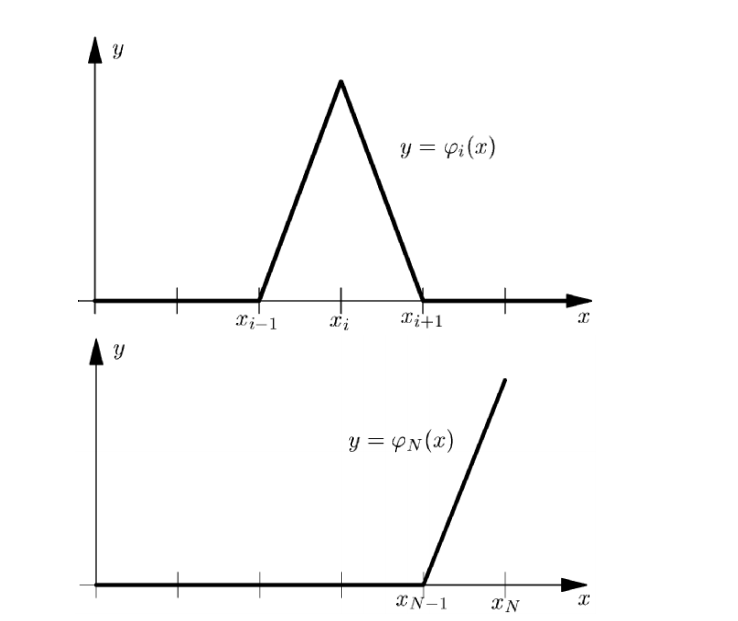
\includegraphics[width=0.6\textwidth]{hatfunction.png}
	\caption{Ansatzfunktionen $\phi_i$ \cite[184]{Numerik}}
	\label{fig:hat}
\end{figure}

Es gilt demnach $\, \, \phi_i (x_k) = \delta_{ik}$ mit  $\, i  ,  k = \, 0 \, , \, 1 \, , \, \dots \,, \,N \,$.
\end{Beispiel}

Nun haben wir eine Idee davon, wie man ein Gebiet zerlegt und wie Ansatzfunktionen aussehen könnten und welche Eigenschaften sie zu erfüllen haben, doch wie genau sieht nun das diskrete Problem bei der \textit{Finite Elemente Methode} nun aus? Dazu müssen wir uns die sogenannte \textit{Assemblierung} der \textit{Steifigkeitsmatrix} $A_n$ anschauen. Wir werden uns die Teilelemente der Zerlegung dazu einzeln anschauen und sogenannte \textit{Elementsteifigkeitsmatrizen} ausrechnen. Im \textit{Assemblierungsschritt} werden wir dann die  \textit{Elementsteifigkeitsmatrizen} zu der \textit{globalen Steifigkeitsmatrix} zusammen setzen.
Wir werden hier nodale Basisfunktionen benutzten. Diese sind durch $\, \varphi_k \, ( \, x_l \, ) = \delta_{kl} \,$ definiert. Weiterhin sei $\hat{N}$ die Zahl der Freiheitsgrade. Rekapitulieren wir das zu lösende Problem

\begin{framed}
\begin{enumerate}
\item $
\text{ Finde ein } u_n \in V_n \text{ : } a(u_n,v_n) = f(v_n) \text{ für alle } v_n \in V_n
$
\item ~Sei $\, \{ \, \varphi_i \, \}_{i=1}^{\hat{N}}$ die Basis  von $V_n$
\item ~Definiere $A_n=( \, a(\varphi_k,\varphi_i) \, )_{i,k=1}^{\hat{N}} \, $ und $ \, f_n=( \, f(\varphi_i) \, )_{i=1}^{\hat{N}}$
\item ~Löse lineares Gleichungssystem $A_n u_n=f_n$ zur Bestimmung der Koeffizienten $u_i$ der Darstellung $u_n(x)=\sum_{i=1}^{\hat{N}} u_i \varphi_i(x)$
\end{enumerate}
\end{framed}

In unserem Fall war $a(u,v)=\int\limits_{\Omega} \Delta u \, \Delta v \, dx \, $ bzw. $\, \, f(v)=\int\limits_{\Omega} f \, v \, dx$. Die zu $\Omega_j$ gehörige Elementsteifigkeitsmatrix besitzt die Form

\begin{equation} \label{eq:element}
\begin{aligned}
A_h^j &= (a_{ik}^j)_{i,k \in I_j} \\
a_{ik}^j &= \int\limits_{\Omega_j} \Delta \varphi_i \, \Delta \varphi_k \, dx \, \, \text{ mit } \, \, 
I_j =\{ i \, : \, supp \, \varphi_i \cap \, \Omega_j \, \neq \emptyset \, \}
\end{aligned}
\end{equation}

Analog dazu die elementweise rechte Seite
\begin{equation*}
f^j = (\, f_i^j \, )_{i \in I_j} \, \, \text{ mit } \, \, f_i^j = \int\limits_{\Omega} \, f \, \varphi_i \, dx 
\end{equation*}

Die globale Steifigkeitstmatrix $A_n$ und die rechte Seite $f_n$ ergeben sich dann wegen der Addivität des Integrals als Summen

\begin{equation*}
A_n = (a_{ik})_{i,k=1}^{\hat{N}} \, \, \, \text{ mit } \, \, \, a_{ik} = \sum_{j=1 \, , \, i \in I_j \, , \, k \in I_j }^M a_{ik}^j 
\end{equation*}

und

\begin{equation*}
f_h = (f_i)_{i=1}^{\hat{N}} \, \, \, \text{ mit } \, \, \, f_i = \sum_{j=1 \, , \, i \in I_j}^M f_i^j
\end{equation*}

$I_j$ ist gerade die List der Eckpunkte der Elemente.
Wir sehen für die Elemente der Elementsteifigkeitsmatrix in (\ref{eq:element}) ein Integral über ein Teilgebiet $\Omega_j$. Hier liegt eine gute Chance viele Operationen zu sparen, indem wir uns die Struktur vom Integral zu nutze machen und mit Hilfe vom Transformationssatz für Integrale eine einheitlichere Form herleiten.

Dazu definieren uns sogenannten \textit{Referenzelemente}. Beispielsweise wenn wir eine Zerlegung in Rechtecken wählen, würden wir uns ein Referenzrechteck definieren oder im Falle von Dreieicken ein Referenzdreieck. Weiterhin definieren wir uns eine lineare Transformation die gerade die Ecken unseres Teilgebiets auf die Ecken des korrespondierenden Referenzelements abbildet. Mit Hilfe vom Transformationssatz formen wir das Integral um und erhalten plötzlich für alle Elementsteifigkeitsmatrizen dieselben Integrale bloß mit verschiedenen Konstanten multipliziert. Die Konstanten sind gerade die Beträge der Determinanten der linearen Transformationen.

Um dann die die Elemente der Elementsteifigkeitsmatrizen in die globale Steifigkeitsmatrix einzubetten, ist dies eine Frage des Umdenkens von einer lokalen Struktur in die globale Struktur.
Dieses Umdenken ist ausschlaggebend für das Verstehen vom Finite Elemente Ansatz und auch der späteren Arbeit zur Herleitung der Pseudoinversen.

Wir rekapitulieren die erste Gleichung dieser Arbeit
\begin{equation} \label{eq:main2}
v=A(u)=\sum_{k=1}^{n_{cells}} C^T P_k^T A_k (P_k Cu)
\end{equation}

Die Variable $n_{cells}$ ist somit die Anzahl der Teilgebiete $\Omega_j$. Die Matrix $A_k$ ist der elementspezifische Operator A. Die Matrix $P_k$ ist genau diese Transformation von der wir gerade sprachen, nämlich die Transformation von den lokalen Freiheitsgraden in die globalen Freiheitsgrade. Es gilt nur noch zu klären, welche Aufgabe die Matrix $C$ in unserer Gleichung besitzt. Diese Frage klären wir im Rahmen des nächsten Unterkapitels zum \textit{Diskontinuierlichen Galerkin-Verfahren}.

Vorher definieren wir uns die Strukturen, die diese Arbeit untersucht. Das ist einerseits die Masse Matrix mit folgender Bilinearform
\begin{equation} \label{eq:mass}
a_M(u,v)= \int\limits_{\Omega} u \, v \, dx
\end{equation}

Eine einfache Struktur, die dazu dient sich an die Thematik ranzutasten und ein Gefühl dafür zu bekommen. Desweiteren wollen wir die Bilinearform des bereits erwähnten elliptischen Problems untersuchen mit

\begin{equation} \label{eq:laplace}
a_L(u,v) = \int\limits_{\Omega} \Delta v \, \Delta v \, dx
\end{equation}

Außerdem brauchen wir etwas Hintergrundwissen, wie wir die Integrale in (\ref{eq:mass}) und in (\ref{eq:laplace}) berechnen können. In der Praxis erfolgt die Berechnung von Integralen über sogenannte \textit{Quadraturformeln}.

\subsubsection{Quadratur}

Allgemein beschäftigt uns das Integrationsproblem
\begin{equation} \label{eq:integral}
I(f) \, = \, \int\limits_{a}^{b} f(x) \, dx
\end{equation}

mit $a,b \in \mathbb{R}$, $\, a < b \, $ und $\, f \in \, C[ \, a,b \, ] $.
Wir werden von interpolatorischen Quadraturformeln gebrauch machen. Intuitiv machen wir eine Polynominterpolation für die zu integrierende Funktion $f$ und summieren über Stützstellen.

Es seien $\, x_i \, \in \, \mathbb{R} \,$, $\, a \, \leq \, x_0 \, < \, \dots \, < \, x_n \, \leq \, b$ Stützstellen mit Gewichten $\, \alpha_i \, \in \, \mathbb{R}$. Dann können wir das Integral (\ref{eq:integral}) approximieren durch

\begin{equation} \label{eq:integral}
I(f) \, = \, \int\limits_{a}^{b} f(x) \, dx \, \approx \, \sum\limits_{i=0}^{n} \, \alpha_i \, f(x_i) \, = I^{(n)}(f)
\end{equation}

Doch wie genau ist diese Approximation? Interpolatorische Quadraturformeln $I^{(n)}(\cdot)$ zu $n \, + \, 1$ Stützstellen sind mindestens von Ordnung $\, n \, + \,1$. Das heißt sie integrieren alle Polynome von maximalen Grad $n$ exakt.

Einer Quadraturformel wollen wir besondere Beachtung schenken, da diese für unsere Anwendung besondere praktikabilität gezeigt hat. 

\begin{Definition} (Gauss Lobatto) \\
Es sei $\, x_i \, $ die $\, (i-1) \,$te Nullstelle des Legendre Polynoms $P^{`}_{n-1}(x)$ und $n$ die Anzahl der Stützstellen, bzw. $n-1$ der Grad unseres Legendre Polynoms. Dann können wir das Integral auf dem Gebiet $[-1,1]$ der Funktion f approximieren durch
\begin{equation*}
\int _{-1}^{1}{f(x)\,dx} \approx {\frac {2}{n(n-1)}}[f(1)+f(-1)]+\sum _{i=2}^{n-1}{w_{i}f(x_{i})}.
\end{equation*}
mit Gewichten
\begin{equation*}
w_{i}={\frac {2}{n(n-1)[P_{n-1}(x_{i})]^{2}}},\qquad x_{i}\neq \pm 1
\end{equation*}
\end{Definition}

Gauss Lobatto liefert uns eine exakte Approximation von Polynomen bis zu Grad $2n-3$. Eine ausführliche  Ausarbeitung der Thematik finden Sie in \cite[79]{Rannacher}.





